\documentclass[a4paper, 12pt]{article}

\usepackage{amsmath}
\usepackage{setspace}
\onehalfspacing
\usepackage{csvsimple}
\usepackage{graphicx}
\graphicspath{{Figures/}}
%\usepackage{floatrow}
\usepackage[%
  font=small,
  labelfont=bf,
  tableposition=top
]{caption}
\usepackage{subcaption}
\usepackage[margin=2.5cm]{geometry}

\usepackage{tabularx}

\usepackage[utf8x]{inputenc}
\usepackage[L7x]{fontenc}

\begin{document}

% [Square brackets are used as indication of temporary text or as comments/notes to ourselves]

\begin{abstract}
We evaluate the Lithuanian support scheme for wind energy deployment, and compare it to the policies in Germany and the UK. This analysis of the Lithuanian support scheme shows that the feed-in tariff system managed to attain low costs. This is achieved by reducing the risks, relative to the Renewable Obligation scheme in the UK. However Lithuania has not achieved as high level of development as Germany, and our survey results from interviewing Lithuanian project developers suggest that the lower development levels is due to: lack of long-term policy commitments, high levels of bureaucracy and difficulties in obtaining finance.
\end{abstract}

\newpage

\tableofcontents

\newpage

\section{Introduction}

In 1990 Lithuania imported 97\% of energy, primarily from Russia. The main objective for the governments in the last two decades has been to increase local production and support energy efficiency (Galinis, Konstantinavičiūtė, Miškinis and Norvaiša, 2011). In 2009 the share of Russian imported energy was down to 56\%, however after December 2009 when the last reactor in Ignalina Nuclear Power Plant in Lithuania was shut down, the Russian share of imported energy shot up to 80\%. In 2004, before the shutting down of the Ignalina Nuclear Power Plant commenced, the power plant had a 41\% share of total installed capacity in Lithuania. Moreover gas imports come from a single source – Russia. The Lithuanian electricity transmission system and the European electricity transmission system is not currently integrated, leaving a limited number of countries where import of electricity is a possibility.

In light of this the National Energy Independence Strategy (2012) has put forward a number of challenges: security of energy supply, competitiveness and sustainability of the energy sector. These challenges are addressed in various ways including: a Liquified Natural Gas terminal (commissioned to open in 2015) that will open the Lithuanian gas market to more suppliers and thereby increase competition, the Visaginas Nuclear Power Plant (commissioned to open in 2020), a Lithuanian-Polish power line LitPol Link (start-up in 2015 and extended in 2020) and a Lithuanian-Swedish power line NordBalt (completed by 2015) that will enable synchronous interconnection between the Lithuanian-Latvian-Estonian electricity transmission system and the European Continental Network, ENTSO-E. Renewable energy is also heavily relied upon as part of the solution. It directly addresses all three challenges. A goal of 23\% renewable energy (20\% renewable electricity) by 2020 has been set.

To support electricity from renewable energy Lithuania introduced feed-in tariffs in 2002. The feed-in tariffs were revised in 2007 and 2009 to adjust for inflation, and again in 2012 where tariffs were differentiated based on the size of the wind farm. Currently feed-in tariffs are calculated using a fixed formula, where net present value of all discounted cash flows should equal zero after 12 years of support, e.g. a break-even point after 12 years. This formula takes into account the amount of invested capital, expected annual quantities of electricity produced, future operational and service costs and the discount rate. This is adjusted according to the specific technology and size of renewable energy plants. National Control Commision for Prices and Energy also adjusts the discount rate using average interest rate for borrowing and lending, corporate tax rate and the 10-year government bond rate average. However feed-in tariff is not differentiated for different regions to account for discrepancy in wind speeds and is set according to an average wind plant efficiency in the country (Feed-in tariff adjustment law, 2011). In 2010 solar photovoltaic was included in the feed-in tariff system. In addition to feed-in tariffs; renewable electricity producers receive a 40\% discount on connection to the grid and the EU Structural Funds provide support for investments in power plants that generate electricity from renewable sources.

\begin{table}
	\csvautotabular{Tables/table_production-electricity-2011.csv}
	\caption{Total gross production of electricity in 2011 in Lithuania}
	\label{tab:table_production-electricity-2011}
\end{table}

% [INSERT TABLE=table_production-electricity-2011.csv TITLE=Total gross production of electricity in 2011 in Lithuania SOURCE=Statistics Lithuania (2012, Table 2.40) Note=* In the combined heat and power plant the fuel is oil and gas. ** Electricity produced using energy from chemical processes.]

Current electricity production in Lithuania is presented in table ~\ref{tab:table_production-electricity-2011}. The majority of production is based on fossil fuel. Hydroelectric plants and pumped storage produced 1.056 GWh (22.5\% of final consumption) in 2011, but further exploitation of hydro is limited: small rivers are already being used, and developing hydro at the bigger rivers Nemunas and Neris is not possible due to environmental issues (Erlickytė, Marčiukaitis and Markevičus 2008). Production from wind turbines has the last couple of years been rapidly increasing and has raised from a production of 224 GWh (4.7\% of final consumption) in 2010 to 475 GWh (10.1\%) in 2011. Electricity from solar plants has so far been negligible, but is likely to increase as developers take advantage of the newly introduced support mechanism. Biomass is undoubtedly the largest renewable energy source in Lithuania, but has not yet been utilised for production of electricity, nor has biogas (Statistics Lithuania 2012). A target of 355 MW by 2020 has been set for biofuel plants. 

The National Energy Independence Strategy sets the total limit of capacity for wind power plants at 500 MW. Galinis et al. (2011, p. 4662) note that capacity above this target ``could have a negative impact on balance of power in the Lithuanian power system and could be a barrier for its planned synchronous operation with ENTSO-E''. Marčiukaitis (2011, p. 4) writes that if the electricity network was expanded the ``real wind energy potential is estimated to reach 1000 MW. Additionally about 1000 MW of offshore wind farms''. Katinas (2007, p. 46) further explains the technical capacity limits for wind power found by the Lithuanian Energy Institute. Currently the system can support an expansion of wind energy up to a capacity of 200 MW without any additional investment. The technical study shows that further deployment up to 500 MW would be achievable with reasonable costs and without causing instability of the system. However this scenario requires a solution to regional differences in the production of wind energy. The coastal region has the greatest potential for wind energy development, but due to weak power connections it cannot bear if all generators are concentrated in this single region. The National Energy Independence Strategy has set these 500 MW as the goal for wind power plants and expects this target to be reached by 2017. 

\subsection{Method, Aim, and Approach}
Butler and Neuhoff (2008) explored the policies promoting wind power development in the UK and Germany from 1990 to 2006. The UK operates under the Renewables Obligation (RO) system which is a tradable green certificate system, while Germany makes use of a feed-in tariff system. Comparing the resource-adjusted cost to society they find that the feed-in tariff system of Germany increases deployment with the lowest cost. Their method of policy effectiveness is based on: the price of power generated, and the capacity installed. The method they apply is similar to the method in the IEA report (IEA 2008), however in the IEA report they also take the countries target levels into consideration when evaluating policy effectiveness, since this makes the comparison unbiased to the country size, starting levels of development and the levels of ambition. The IEA report also finds that the UK in 2004/5 is approximately 30\% more costly per kWh than Germany, and yet its policy effectiveness score for onshore wind power generation is 1/4 of the German.

In addition to comparing costs and development levels, Butler and Neuhoff conducted a survey among project developers. The survey they use to uncover developmental barriers intrinsic to the support mechanism and extrinsic to it, the level of competition among wind developers and among suppliers to wind developers. They find that project developers in Germany compete for good sites rather than on price, since ``the tariff adjusts to the available wind resource, it allows developers to pursue projects in a wider set of locations'' (Butler and Neuhoff 2008, p. 1860).

Since the publication of their paper there has been some changes to the UK and German support policies. In 2010 the UK implemented feed-in tariffs that works alongside the RO system. The feed-in tariffs are aimed at increasing development of small-scale generators (less than 5 MW), while the focus of RO is still development of large-scale generators. Solar photovoltaic has dominated the first year of instalments with 77.7MW, four times more than, the second most installed, wind at 18.9MW (Ofgem 2011). In 2009 repowering bonuses were introduced in Germany when replacing old wind turbines (pre-2002 constructions) and tariff rates were adjusted (EEG, 2009). And from 2012 Germany guarantees small-scale turbines (less than 50 kW) their high tariff rate for 20 years, instead of the 5 years guaranteed for large-scale turbines, and rates were adjusted again (EEG 2012). This paper will only consider large-scale generators, and there ignore these recent updates to the support mechanisms when doing price comparisons.

In this paper our approach is to extend the comparative analysis of the resource adjusted cost to include Lithuania, and in doing this we will provide the reader with a policy effectiveness evaluation of the feed-in tariff system of Lithuania, relative to Germany and the UK. We compare to another feed-in tariff system, but also compare with a green certificate based system. To account for differences in country size and starting levels of development we will also include the method from the IEA report (IEA 2008). And we will supplement the policy effectiveness evaluation with a survey among lithuanian project developers that will uncover the barriers that might have limited wind energy development in Lithuania. 

But why Lithuania, you might ask. Because Lithuania shares the characteristics of the majority of other countries in the world. Lithuania has some special limitations and features that translate quite easily to a lot of other countries; it is at a very early stage of wind power development and an early stage of creating effective policy incentives. It is a small country where low wind speeds in one part of the country are not simply compensated by high wind speeds in another part. It is not yet integrated into a large electricity transmission system and finally it is a small economy where it’s investment and remuneration levels are constrained by its resources. We can therefore motivate the choice of Lithuania by it being a representative country and that the methods and conclusions presented here might serve other countries sharing the characteristics listed above.

\section{Policy efficiency}
We will first have a look at development levels, thereafter introduce the respective wind resources or wind speeds in each country, which we later will use to adjust costs. We will calculate the value of ROC for later use. And end up evaluating costs or remuneration levels to see if the findings of different deployment levels are a result of the different remuneration levels when these have been adjusted for the wind resources of each country.

\subsection{Comparing deployment level}
\begin{figure}
	\centering
	%\begin{subfigure}[b]{0.2\textwidth}
	%	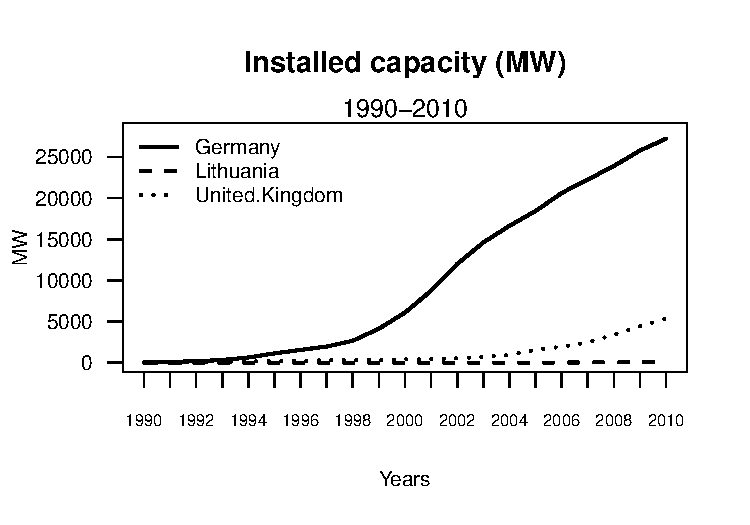
\includegraphics[width=1\textwidth]{figure_capacity}
	%	\caption{Installed wind power capacity 1990-2010 (MW)}
	%	\label{fig:figure_capacity}
	%\end{subfigure}
	%~
	\begin{subfigure}[b]{1\textwidth}
		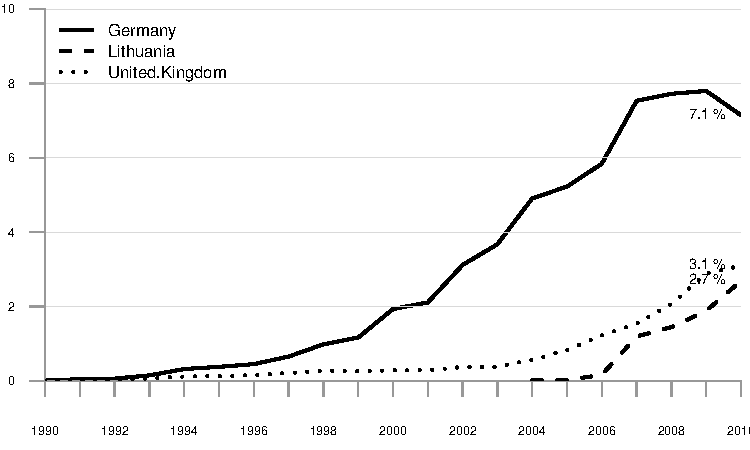
\includegraphics[width=1\textwidth]{figure_generation-share2}
		\caption{Wind power share of final consumption (\%)}
		\label{fig:figure_generation-share2}
	\end{subfigure}
	~
	\begin{subfigure}[b]{1\textwidth}
		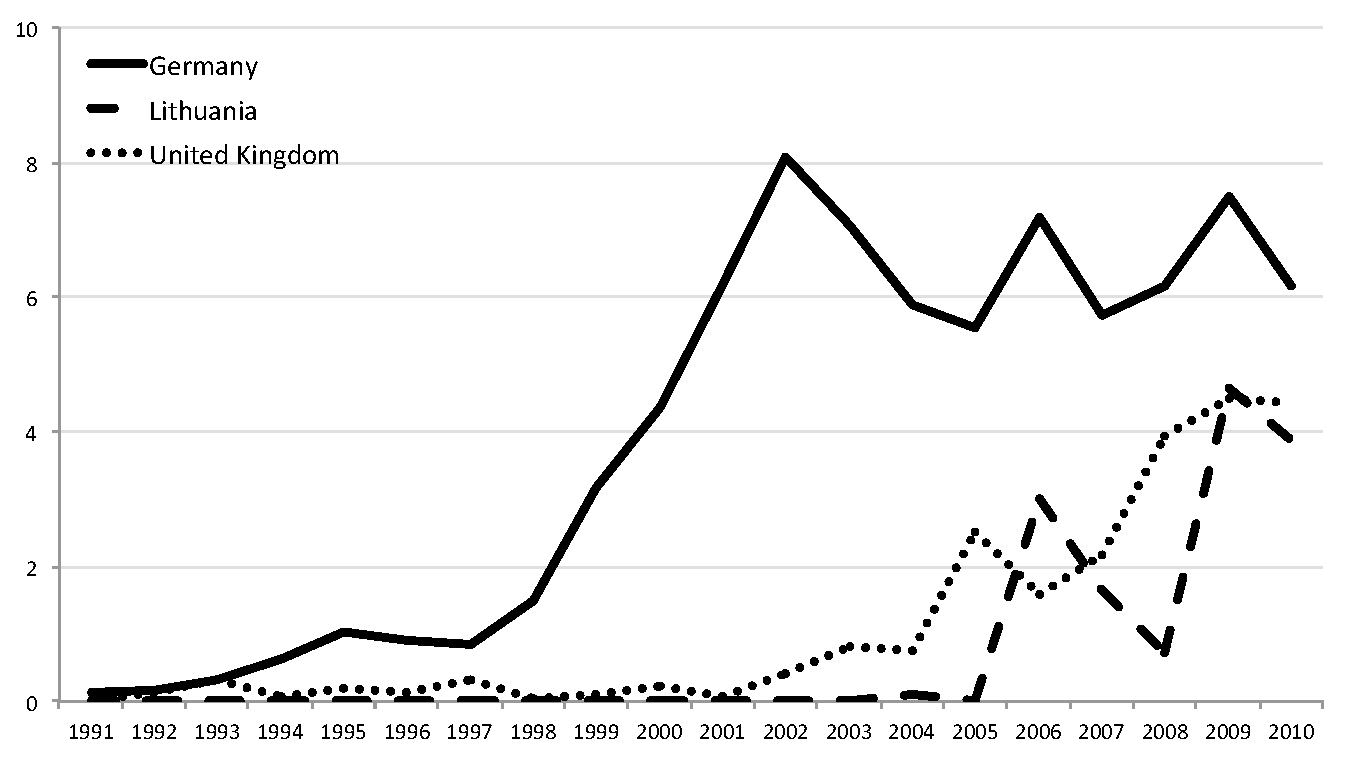
\includegraphics[width=1\textwidth]{fig_growth-potential}
		\caption{The annual additional capacity growth share of remaining additional mid-term realisable potential (\%)}
		\label{fig:fig_growth-potential}
	\end{subfigure}
\end{figure}
% [INSERT FIGURE=figure_capacity.pdf TITLE=Installed wind power capacity 1990-2010 (MW) SOURCE=EUROSTAT (nrg_113a) TIME=1990-2010 NOTE=Includes both onshore and offshore wind turbines. Sum of main activity producers and autoproducers]

% [INSERT FIGURE=figure_production_share2.pdf TITLE=Wind power share of final consumption (\%) TIME=1990-2010 SOURCE=Eurostat (nrg_113a) NOTE=Includes both onshore and offshore wind turbines. Sum of main activity producers and autoproducers]

% [INSERT FIGURE=... TITLE=The annual additional capacity growth share of remaining additional mid-term realisable potential (\%) TIME=1990-2010 SOURCE=Eurostat (nrg_113a). EWEA (2012) NOTE=Includes both onshore and offshore wind turbines. Sum of main activity producers and autoproducers]

Both Germany and the UK introduced renewable energy incentive policies around the same time, in 1991 and 1990 respectively. Deployment has been much greater in Germany compared to the UK. In Germany deployment increased steadily after the first national policy was introduced incentivising electricity production from renewable energy sources. The capacity growth rate has stabilized in the last couple of years. Deployment in the UK remained low under the NFFO system and only started to pick up after the RO system was introduced in 2002, but both the NFFO and RO have under-performed with regards to the targets set by government (Dow and Wood 2011, table 2.1). Lithuania has arrived much later at the game. First introducing feed-in tariffs in 2002. Its deployment in absolute terms (MW) has been slower than both Germany and the UK. However the rate at which wind power as percentage of final electricity consumption has increased, has been faster as seen in figure ~\ref{fig:figure_generation-share2} – reaching a 2.7\% share of final consumption in its first 8 years. This is most likely due to catch-up effects: e.g. better technology has been available at the time when Lithuania finally introduced its renewable energy policy. We will use the IEA effectiveness indicator method (IEA 2008) to take account of this, and calculate the annual additional capacity growth rate as a percentage of the remaining additional mid-term realisable potential, were respective 2020 capacity targets for each country has been used\footnote{The equation is $E_t = \frac{G_t - G_{t-1}}{\text{ADDPOT}_t} = \frac{G_t - G_{t-1}}{\text{POT}_{2020} - G_{t-1}}$, where E is the effectiveness indicator, G is capcity in year t, ADDPOT is additional potential in year t until 2020, and $\text{POT}_{2020}$ is capacity potential in year 2020.}.  Doing this we see that the growth rate is largest in Germany and has been stable at an annual growth of 6.5\% of additional potential, the last ten years (figure ~\ref{fig:fig_growth-potential}). While Lithuania and the UK have lower, very similar and continually increasing growth rates. Despite the UK having a 10 year renewable policy head start, and having higher potential in the form of higher average wind speeds as we will see in the following section, its current level of development is similar to the level in Lithuania.

\subsection{Comparing wind speeds and wind resources}

\begin{table}
	\begin{tabular}{|p{2cm}|p{3cm}|p{2cm}|p{2cm}|p{2cm}|p{3cm}|}
	  DE & LT & LT & LT & LT & UK \\
	  Reference site & Average of test sites (Vilkyciai, Kretinga, Tauragè) & Giruliuose & Būtingėje & Coastal region * & Existing wind farms ** \\
	  5.5 & 6.06 & 5.95 & 6.88 & 7.23 \\
	\end{tabular}
	\caption{Comparable average wind speeds at height of 30 m (m/s)}
	\label{tab:table_avgwindspeeds}
\end{table}

% [INSERT TABLE=table_avgwindspeeds.csv TITLE=Comparable average wind speeds at height of 30 m (m/s) SOURCE=UK: Butler and Neuhoff (2004, p. 13). DE: IEA (2000, p. 96). LT: Marciukatis (2011), Erlickytė-Marčiukaitienė, Marčiukaitis and Tumosa (2007, p. 27) NOTE=LT and UK wind speeds have been calculated at 30 m using the wind gradient equation with a Hellman exponent of 1/7. * Wind speeds from hydrometeorological stations measured at 10 m above ground. ** Wind speeds calculated using the DTI NOABL database.]

To accurately compare the costs in Germany, the UK and Lithuania we will adjust costs according to each countries wind resources. Germany is endowed with the lowest wind speeds and therefore its costs of producing one MWh will be higher than the UK and Lithuania. 

Butler and Neuhoff (2004, p. 13) reports that the UK wind speeds at existing wind farms is 7.04 m/s at a height of 25 m, which corresponds to 7.23 m/s at a height 30 m. Wind speeds for Lithuania and the UK have been calculated such that they are comparable to the 30 meter height of the German reference site. This is presented in table ~\ref{tab:table_avgwindspeeds}\footnote{Wind gradient equation: $\text{V}_h = \text{V}_\text{30m} \cdot \left(\frac{h}{30}\right)^\alpha$ where $\text{V}_\text{30m}$ is the wind speed at a height of 30 meters,, $\text{V}_h$ is wind speed at height of $h$ meters, and where  $\alpha$ is the Hellman exponent, that accounts for the terrain and roughness.}.

There is no agreement upon the average wind speed for Lithuania, nor any database containing wind speeds for the existing wind turbines, therefore we present the wind speeds of five sites, and wind speed for the Coastal region. The wind speeds of the three test sites (Vilkyciai, Kretinga, and Tauragè) are the result of the Baltic wind atlas study by RISØ (2003). They furthermore (using data from met-office stations) provide readers with a map approximating how the wind speed decreases as you travel east over Lithuania away from the Baltic sea. Similarly Erlickytė-Marčiukaitienė, Marčiukaitis and Tumosa (2007, p. 27) report wind speeds for the Coastal region, calculated using data from hydrometeorological stations. They also report that the lowest wind speeds are found in the eastern and southeastern parts of Lithuania. Here wind speeds fall below 2.5 m/s at 10 m (corresponding to 2.9 m/s at 30 m). Marčiukatis (2011, p. 4) reports that ``measurements carried out during a number of private wind energy projects have shown even better wind conditions [than the three test sites mentioned above]. Unfortunately, they are confidential and not available for presentation''.

Power production increases proportional to the wind speed cubed (Danish Wind Industry Association, 2012. Grogg 2005, eq. 2). We can very roughly assume that a UK turbine will approximately achieve 227\% of the output that the same turbine would achieve at the German reference site, while a Lithuanian turbine will achieve 127-196\% of the German reference site\footnote{Calculated as: $\frac{\text{P}}{\text{P}_\text{DE}} = \frac{\frac{1}{2} \cdot A \cdot \rho \cdot \text{V}^3}{\frac{1}{2} \cdot A \cdot \rho \cdot \text{V}_\text{DE}^3} = \left(\frac{\text{V}}{\text{V}_\text{DE}}\right)^3$, where $A$ is area of disk where air flows through, and $\rho > 1$ is density of air. These two parameters are  assumed to be identical in all three countries.}.

It is important to note that neither the NFFO or RO in the UK, nor the feed-in tariffs in Lithuania, differentiate with respect to wind resources\footnote{Lithuania tariffs will most likely be differentiate with respect to wind resources as a result of a forthcoming auction system, where developers submit regional bids (see more on this in a later section)}. While the German feed-in tariffs from 2000 and onwards offer higher tariffs for less windy sites\footnote{High performing sites reaching 150\% of the performance of a reference site receive 9.1-7.9 c/kWh for five years and thereafter 6.2-5.4 c/kWh. While for low performing sites the 9.1-7.9 c/kWh rate is extended after the 5 years, by two months for every 0.75\% the low sites are below the 150\% reference site. These rate were revised in 2004, 2009 and 2012 (Lauber and Mez 2004. EEG 2012).}. This is important since it has implications for the order in which different sites/regions are developed and their profitability. When tariffs are not differentiated, the least favorable site sets marginal price. In the beginning, when installed capacity is low, project developers will focus on the sites with high wind speeds. As deployment expands, sites with increasingly lower wind speeds will be used, and the increased remuneration levels required at these sites will set marginal price. This leads to the turbines located at the high wind speed sites capturing scarcity rents. By differentiating tariffs according to the wind resources available, high scarcity rents can be avoided. Huber, Ragwitz, Resch, White (2003 table 3.25) estimated that in 2001 Germany had achieved 26\% of its mid-term potential electricity generation from onshore wind power, while the UK had only achieved 4.1\%. Indicating that the UK was still far from a level of deployment where we could talk about scarcity, while the measure against scarcity rents is more relevant in Germany.

\begin{figure}
	\centering
	%\begin{floatrow}
		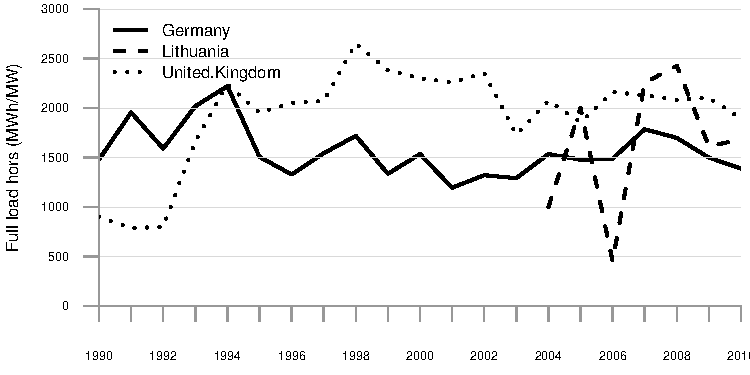
\includegraphics[width=1\textwidth]{figure_generation-capacity}
		\caption{Generation from installed capacity lagged one period (MWh/MW)}
		%\floatfoot{Includes both onshore and offshore wind turbines. Sum of main activity producers and autoproducers}
		%\figsource{Eurostat (nrg_113a, nrg_1072)}
		\label{fig:figure_generation-capacity}
	%\end{floatrow}
\end{figure}
% [INSERT FIGURE=figure_generation-capacity.pdf TITLE=Generation from installed capacity lagged one period (MWh/MW) TIME=1990-2010 SOURCE=Eurostat (nrg_113a, nrg_1072) NOTE=Includes both onshore and offshore wind turbines. Sum of main activity producers and autoproducers]

Following the procedure of Butler and Neuhoff (2008, 2004) we will not use country average wind speeds, since they might not correspond to wind speeds at the sites, that are accessible to project developers. Instead we will look at the electricity generated relative to the installed capacity (MWh divided by MW). This measure is also called the annual full load hours (h/a), since it corresponds to the number of hours where a wind turbine has to produce at its maximum capacity. This will serve as a crude measure of the output of all operational wind turbines. 

Figure ~\ref{fig:figure_generation-capacity} presents the electricity production from the installed capacity. Because of the better wind resources we see (as expected) that output is higher in the UK compared to Germany, with exception of the early 1990s. Butler and Neuhoff (2008, p.1858) explains that this initial lower output in the UK was ``due to low turbine ratings at experimental sites, but increased with the increase in turbine rating throughout the 1990s'' and they further note that the ``increase in hub height – thus capturing higher wind speeds – has contributed to the upward trend in the UK and has prevented a further decrease in output per turbine in Germany''. Caution is advised when evaluating the output of Lithuania in 2004-2005, since the numbers are very sensitive to rounding and measurement errors\footnote{Capacity was reported to be 1 MW in both years, while electricity generated was reported respectively as 1 and 2 GWh in those years by EUROSTAT. The National Control Commission for Prices and Energy reported that they had issued permits that cumulative had capacities of 0.85 and 0.99 MW (NCC 2006, table 41), while the European Wind Energy Association reports installed capacity of 7 MW in both years (EWEA 2006). Statistics Lithuania report electricity generated as 1.2 and 1.8 GWh (Statistics Lithuania 2006).}. After 2006 the Lithuanian output is situated in the vicinity of UK output, which probably reflects that wind deployment has currently taken place in the locations where wind resources are highest, rather than evenly distributed across Lithuania. Our output measure might further decrease, as high resource locations become scarcer and development moves to less windy sites. In addition, within a couple of years, Lithuanian output will most likely stabilize somewhere in between the German and UK levels – like we have seen German and UK output levels stabilizing after half a decade or so of initial development. 

We will leave development levels and wind resources for now, and concentrate on the costs of the different support mechanisms, but will return later when we calculate the wind resource-adjusted costs and compare these to the levels of deployment that the countries have achieved.

\subsection{The value of ROCs}

We will now take a closer look at the prices paid for wind energy; first calculating the value of ROC in the UK, thereafter comparing prices across countries taking wind resources into account. Butler and Neuhoff (2008, p. 1855) choose to focus on the cost per kWh of wind energy, rather than on the overall cost of support, since ``the overall cost would also include network expansion costs and balancing costs, to which wind generators in Germany are not exposed, and which can be separated in the UK''. Similarly we will focus on the unit cost, since as mentioned earlier, Lithuania is also constrained by a network capacity (500 MW) and attendant expansion and balancing costs.

\begin{figure}
	\centering
	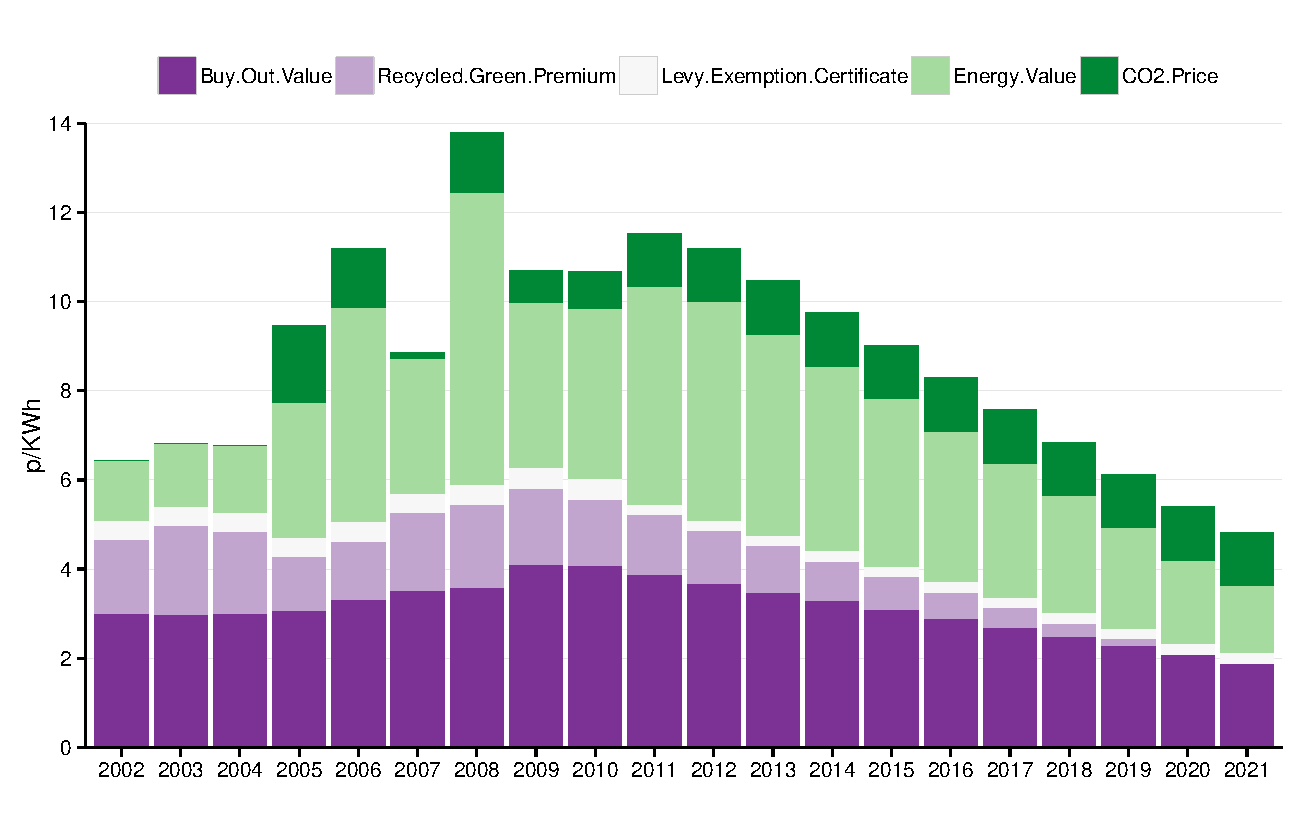
\includegraphics[width=1\textwidth]{figure_roc-price-components}
	\caption{Components of the Price Paid to Wind Energy under ROC (p/kWh)}
	\label{fig:figure_roc-price-components}
\end{figure}
% [INSERT FIGURE=figure_roc-price-components.pdf TITLE=Components of the Price Paid to Wind Energy under ROC (p/kWh) TIME=2002-2021 SOURCE=… NOTE=… ]

The UK's Tradable Green Certificate are called Renewable Obligation Certificates (ROCs). Energy suppliers have to present a certain number of ROCs each year (11.1\% of total electricity supplied in 2010/2011), this is monitored by Ofgem. ROCs can be bought from renewable energy generators (1 ROC = 1 MWh). The value of ROCs is not simply equivalent to the market price of the traded ROCs, since the RO system also allows suppliers to pay a fixed amount (buy-out price) to Ofgem for each MWh above the requirement, that they have not covered with a Renewable Obligation Certificate. Other factors of the RO system also affect the value of ROCs as we will see below.

When calculating the value of ROCs we will follow the approach first presented by Bauknecht, Connor and Mitchell (2006). This is also the approach taken by Butler and Neuhoff, but we have updated several assumptions to fit the newest projections and price developments. Like them we aim at providing a lower bound of the value of ROCs, since we are optimistic about renewable energies and because we assume that UK investors are conservative in their expectations.

The buy-out price was set at £30/MWh (= 3 p/kWh) in 2002/2003, when the RO system was introduced and it increases annually with the Retail Price Index\footnote{The buy-out price also works as a cap on RO expenditures. It insures that consumers will not pay more than 3 p/kWh on a fixed \% of their electricity (Bauknecht, Connor and Mitchell 2006, p. 300)}. The electricity suppliers have an economic interest in buying renewable energy up to £30/MWh above the market price of conventional electricity. If the electricity price of renewables was above, then suppliers would instead buy conventional electricity from the market, and pay the buy-out price. In line with Butler and Neuhoff we assume that from 2010 the buy-out price falls with technology (0.20 p/kWh annually), see figure ~\ref{fig:figure_roc-price-components}.

The buy-out funds collected each year are redistributed to those suppliers that have met their requirements. These recycled funds further increase the premium above market price, at which suppliers are willing to buy renewable energy, and hence increase the value of ROCs. This is denoted Recycled Green Premium in figure ~\ref{fig:figure_roc-price-components}. Butler and Neuhoff assumed that the UK would meet their renewable energy targets in 2010/2011 and that the recycled green premium thereafter would simply be zero. As noted earlier the UK has consistently under-performed with regards to the targets set by the government. We will instead assume the target will not be meet before 2020, and the premium will fall until then. This seems reasonable given that 71\% of all producers met their target in 2010/2011, up only by 15\%-points in 7 years (Ofgem 2008, table 1. Ofgem 2011, table 1.) 

Levy Exemption Certificate (LEC) exempts renewable energy generators from the Climate Change Levy. Butler and Neuhoff assumed this to be fixed at 0.22p/kWh (50\% of the 2007/2008 level). We use the actual rate for the first 10 years and then assume the future rate will remain at 50\% of the 2010/2011 level.

The ROCs are an additional revenue source for renewable energy generators, but like all energy generators the energy they produce is sold to the market and constitutes their primary revenue source. We calculate the energy value as the auction price for wind in the NFPA auction, minus the ROC auction price and the value of LEC\footnote{The auction prices for wind will include the value ROCs and LECs (NFPA 2012).}. In line with Butler and Neuhoff (2008, p. 1857) we assume that the energy value falls with technology (to 1.5p/kWh in 2020), since this is the ``bottom end of the range predicted by the Performance and Innovation Unit''.

In 2005 the European Emission Trading Scheme was introduced. It increases the fossil fuel (opportunity) cost of electricity generation, this is denoted \emph{CO2 prices} in figure ~\ref{fig:figure_roc-price-components}. From 2007 and on, Butler and Neuhoff in their calculations assume a fixed CO2 price of 22.77 €/tCO2, but since then the CO2 price has fallen from a levels around 20 and 22 €/tCO2 (in 2005 and 2008) down to 7.5 €/tCO2 in 2012\footnote{The Committee on Climate Change (2008, p. 149) write that the CO2 prices fell to zero in 2007 due to an oversupply of total permits issued in Phase I. And that the prices fell after 2008 because of expectations regarding the banking arrangements between Phase II and III.}. We will base our assumption on the central case price projection made in the Committee on Climate Change report (2008, p. 162). They set prices at 16 €/tCO2 in 2020, and only slightly lower in 2015. We assume a fixed cost of 16 €/tCO2 this corresponding to a contribution of 1.2 p/kWh each year\footnote{In addition we also assume an exchange rate of 1.5 and a conversion factor of 0.5 corresponding to the latest available level (2010 level).}.

By taking advantage of newest available data and updating the assumptions we find that the sum of all ROC components is higher than the value Butler and Neuhoff (2008) found. This of course also leads to the compounded UK prices being considerably higher. The calculation will appear in the coming sections. 

Above we briefly described each ROC component as well as its past and future price developments. The sum of all components gives us an projection of what the ROC value wind producers in the UK can expect in each year until 2021. Using this and the tariff rates from Germany and Lithuania we will be able to make a simple inflation adjusted price comparison for the years 2002-2021 – this is done in the following section. And later extended with the elaborate price comparison were also wind resources are taken into account.

\subsection{Expected average remuneration under the EEG and the RO}
\begin{figure}
	\centering
	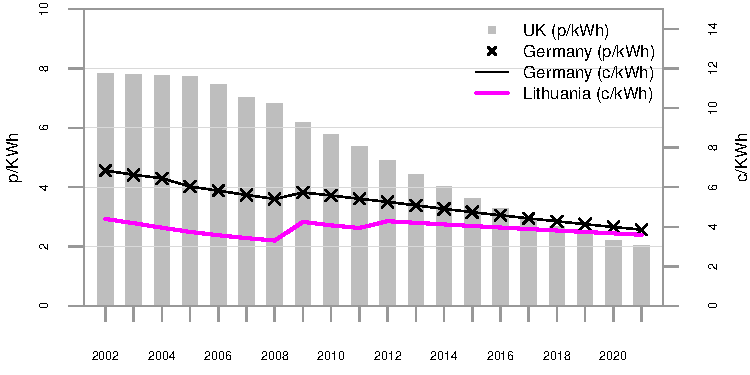
\includegraphics[width=1\textwidth]{fig_expected-average-remuneration-priceadjusted}
	\caption{Expected remuneration level (2002-2021)}
	\label{fig:fig_expected-average-remuneration-priceadjusted}
\end{figure}
% [INSERT FIGURE=fig_expected-average-remuneration-priceadjusted.pdf TITLE=Expected remuneration level (2002-2021). TIME=2002-2021 SOURCE=… NOTE=… ]

In this section we will calculate remuneration levels that are comparable across the three support mechanisms, despite the fact that prices, rates and the length of support differs widely in each system. The procedure is as follows: we will calculate the net present value of a newly build wind turbine for each year from 2002 to 2021. We assume a discount rate of 8\% and payback time of 20 years, e.g. we evaluate the investment by looking at the cash flow in the first 20 years after the turbine has been built. Furthermore before calculating the net present values, we deflate the cash flow with respect to the respective retail price indices (2003=100), producer price index is used in Lithuania, and for the year 2011 and thereafter we assume a constant annual inflation rate of 1.96\% for all three countries in line with the ECB target of just below 2\%. Then we calculate constant annual rates that would yield identical net present values, since this rate or remuneration level for each year will be comparable across the three systems, and takes account of the system differences mentioned above. The results of this procedure is presented in figure ~\ref{fig:fig_expected-average-remuneration-priceadjusted}. We use a fixed GBP-EUR exchange rate of 1.5 in this and next figure.

In the UK we use the value of ROC that we calculated in the previous section. For each year between 2002-2021 we use the corresponding ROC value. For years after 2021 we simply assume a constant value of 3 p/kWh\footnote{Butler and Neuhoff (2008) calculate ROC values until 2024 and assume a constant price of 2.79 p/kWh from 2025 and on.}.

In Germany we assume that wind turbines are located at windy sites and produce at 150\% above the reference site. They are therefore eligible for five years high initial fee followed by 15 years of basic fee. We also apply the degression mechanism of the EEG system. It decreases initial and basic fees for new builds with 1-2\% annually. The EEG system has been revised three times since it was introduced; in 2004, 2009 and 2012 - each revision has adjusted fees and degression rates.

In Lithuania the feed-in tariff rates have been adjusted twice since its introduction - in 2009 and 2012. The rate was 6.37 c/kWh until 2009 when it was increased to 8.69 c/kWh\footnote{We assume a fixed LTL/EUR exchange rate of 63.7/220 ≈ 0.2895 similar to Marčiukaitis (2011).}. The 2012 adjustment introduced differentiated tariffs based on the size of the wind project: for projects smaller than 30 kW the offered tariff is 10.71 c/kWh, between 30 kW and 350 kW the tariff is 10.42 c/kWh, and above 350 kW the tariff is 8.11 c/kWh. To this date, only two wind projects below 30 kW have been developed; moreover mid-size projects account for 68\% of all projects while large-sized project account for 29\% (NCC 2012). It is too early to predict the future distribution and the size of wind projects. Therefore we use the simple average of these three rates, and set the price to 9.75 c/kWh from 2012 and onwards\footnote{A weighted average, where weights are the current number of projects in each size, increases the price with 0.25 c/kWh.}. 

In Lithuania renewable energy producers are guaranteed the feed-in tariff rates for 12 years. After 12 years we assume that producers are paid the pool price. On the 1st of January, 2010 the Lithuanian electricity power exchange (Baltpool) opened. This and the final closing of the Ignalina nuclear power plant by 31st December, 2009 substantially affected the wholesale electricity market. Before, prices had been stable for 10 years at levels around 1.9 c/kWh (NCC 2006, p.12 ). For 2010-2012, we have calculated an average price of 4.56 c/kWh using data from Baltpool (2012). Even though Lithuania has seen a jump in prices and future prices remain uncertain due to the possible commissioning of a new nuclear power plant, we will assume that the pool price in Lithuania is equal to the average Baltpool price, and will remain so in the future. When Lithuania joined the EU in 2004, it committed to closing the Ignalina Nuclear Power Plant, and liberalizing the electricity market. We assume that project developers believed this government commitment and therefore foresaw the higher pool price. In addition to that we also assume that even if a new nuclear power plant is built, it will not be able to influence future market price, as Lithuania by then will be part of a larger transmission system.

This simple comparison of remuneration levels reveals that ROC remuneration levels are considerably higher than EEG levels and presumably will remain higher until the mid- to late-2010s. Butler and Neuhoff (2008) estimated ROC remuneration levels that stayed below 7 p/kWh. Our estimates are significantly higher due to the UK not reaching their target levels and therefore the recycled green premium has not yet converged to zero, and due to wind energy auction prices in 2008 being 2 p/kWh higher than their estimate. We also see that the Lithuanian remuneration levels are lower than the German levels, and presumably will remain lower until 2020. This will however depend on the relative future inflation levels – in non-price-adjusted terms the Lithuanian remuneration has been higher than the German since 2009. This simple comparison though insightful, does not take the wind speeds into account. In the next section we will make this adjustments and compare the prices for years 1990-2010.

\subsection{Anticipated price of wind energy in Germany and the UK}

\begin{figure}
	\centering
	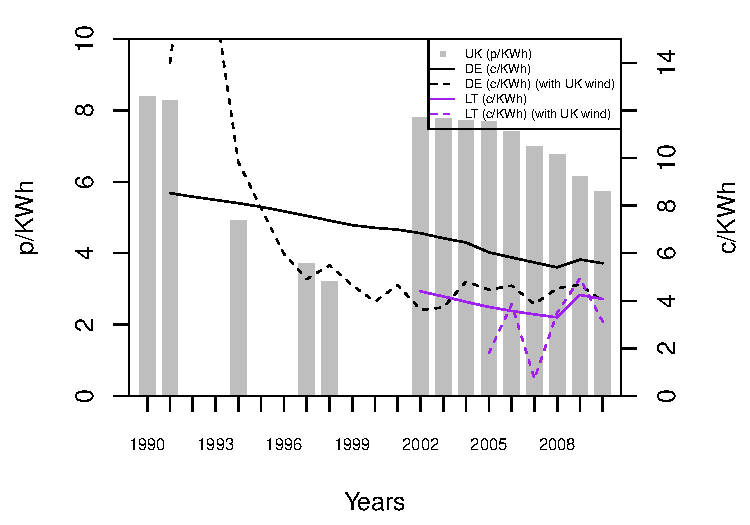
\includegraphics[width=1\textwidth]{fig_anticipated-price-energy}
	\caption{Anticipated price of wind energy (1990-2010)}
	\label{fig:fig_anticipated-price-energy}
\end{figure}
% [INSERT FIGURE=fig_anticipated-price-energy.pdf TITLE=Anticipated price of wind energy (1990-2010). TIME=1990-2010 SOURCE=… NOTE=… ]

In this section we have applied the procedure from the previous section to the deflated NFFO auction prices and the StrEG prices; calculating the net present values for each year, and thereafter a corresponding constant remuneration level. In addition we also use the remuneration levels calculated in the previous section for years 2002-2010 (2000-2010 in the case of Germany). But in this section we take account of different wind speeds, as Butler and Neuhoff (2008, p. 1858) write ``If, for example, output [of wind turbines in the UK] is 20\% higher, then the price paid per MWh can be reduced by 20\% [in Germany …] maintaining the same revenue stream for the project and creating little additional maintenance costs''. When adjusting for UK wind speeds we multiply remuneration levels with the full load hours divided by the full load hours in the UK – our crude measure of output from a previous section (see figure ~\ref{fig:figure_generation-capacity})\footnote{Calculated as $\text{PMT}_\text{UK Wind} = \text{PMT} \cdot \frac{\text{MWh}}{\text{MW}} \cdot \left(\frac{\text{MWh}_\text{UK}}{\text{MW}_\text{UK}}\right)^{-1}$ where PMT is the constant rate, giving the same NPV}.

Five NFFO auction rounds were completed before the ROC system was introduced in 2002. NFFO 1-2 guaranteed the NFFO auction price until 1998, while the NFFO 3-5 guaranteed prices for 15 years, for each year after the support expired we assume wind turbines receive an annual pool price of 1.5 p/kWh. 

The StrEG system was introduced in 1991 in Germany, and guaranteed renewable energy producers 90\% of final consumer electricity prices\footnote{Electricity transmission system exhibited significant loss as electricity is transmitted from power plants through the grid to final consumers. Therefore the prices final consumers will pay when they draw electricity from the grid is much higher than the price that (non-renewable) producers receive when delivering electricity to the grid. The 90\% will therefore give renewable energy producers a premium relative to non-renewable.}. For each year we use the corresponding StrEG price. For the years after 2000, where the StrEG system has been replaced by the EEG system, we assume four years of a high initial fee (similar fees as in year 2000), followed by the basic fee for remaining years\footnote{This is similar to, but not mentioned in, Butler and Neuhoff (2008) and has been found by method of trial-and-error, using hints from the EEG law (2000) where it is stated that operation time of prior installation is halved (but to minimum 4 years) and after that prior installation follow same reduction of rate rules as new installations.}.

Butler and Neuhoff (2008) conclude that although the the NFFO and RO system was theoretically thought of as systems that effectively reduced costs through price competition, when the period of support, inflation, and wind resources are taken into account, this does not seem to be the case. Germany has been able to reduce price just as well, through a feed-in tariff system where no price competition exists. In addition to cost reduction, the NFFO system suffered from several problems, as discussed in Mitchell (2000), Connor and Mitchell (2004) and Dow and Wood (2011). If we look at the period from 2002 when the RO system was introduced, costs have still been lower in Germany compared to the UK. Bauknecht, Connor, and Mitchell (2004) argue that a feed-in tariffs system reduces risks better than the RO system. They conclude that the German feed-in tariff system has been more effective by lowering price-, volume- and balancing-risks; Lowering price risks by providing a fixed rate. Lowering volume risks by guaranteeing producers to buy all the electricity they produced. And lower balancing risks by fixing the remuneration level irrespectively of the load profile, while the New Electricity Trading Arrangements in the UK ``places a high premium on flexibility and penalises unreliable generation'' (Bauknecht, Connor, and Mitchell 2004, p. 301). Dow and Wood (2011, p. 2229) go further and argue that the replacing RO system introduced three new failures, while it only managed to remove the problem of renewable energy subsidies being bundled together with nuclear energy subsidies. They describe an additional seven system failures of the NFFO system that the RO system has not yet corrected.

While Lithuanian remuneration levels have changed relatively few times, and therefore  has been quite stable, the inflation adjusted comparison of prices paints a different picture. Lithuania has experienced relatively unstable inflation levels, compared to the UK or Germany. When adjusting for wind resources we see that prices are quite similar to German prices. Again caution is advised when evaluating 2004 and 2005 in Lithuania, as it might easily be subject to rounding and measurement errors. Feed-in tariff systems keep support costs low, since it reduces risks. We find that this is the case irrespectively of the specifics of the system, such as the period of support or differentiating the tariffs based on wind resources. Lithuania has taken advantage of this low cost system, and managed to have development levels comparable to the UK. But the development levels have not been as large as in Germany, we believe this is not due to the specifics of the feed-in tariff system but to other factors, unrelated to the support mechanism. We will try to uncover these in the next section where we present the results of our survey among Lithuanian project developers.

\section{Survey}
From the beginning of our project we had an idea that not only the financial support scheme matters for the policy to be effective. Our initial thoughts were supported in the IEA report (2008, p.100) where they emphasize that non-economic barriers can be the cause of slow renewable energy deployment. In addition to that, Galinis et al. (2011, Section 3.2) also stated their concerns that in Lithuania, there exists more than financial and technical barriers to entry. And as argued by Sawin (2004) these additional barriers can have a huge impact on policy effectiveness.

We have adapted the survey questions from Butler and Neuhoff (2008) so that they fit the current Lithuanian situation. The questions where project developers to give a score, are unchanged such that the results are comparable to Butler and Neuhoff’s, but the open ended questions have been changed. We used this method to examine barriers to entry in Lithuania and competition between wind energy developers and their suppliers. In addition to that we extended the questionnaire to uncover current attitude towards the feed-in tariff system and the risks as seen from the perspective of project developers.
 
We collected responses from 7 Lithuanian developers who account for 11 working projects, out of a total of 41 projects currently running in Lithuania (NCC 2012). Project developers were found using the NCC (2012) list of supported producers. Our survey results are presented alongside the survey results of Butler and Neuhoff (2008), who received response from 10 UK developers and 13 German, further note that their survey was conducted in 2004.

\subsection{Barriers}
In this section we will provide our results on the difficulties experienced in each stage of development. And relate the responses to the problems in Lithuania noted by Marčiukaitis (2011) and the policy effectiveness requirements and recommendations made by Sawin (2004). Project developers were asked to evaluate the difficulty of each stage on a scale from 0 to 5 – where 0 means no difficulty and 5 is major difficulty. Moreover we collected additional comments about the difficulties in each step during the planning process and will report them alongside the numerical scores of the survey, see fig ~\ref{fig:fig_survey_barriers}.

The overall rating for difficulties encountered during different stages of development was 3.4 in Lithuania. Which is much higher than what Butler and Neuhoff found in Germany (2.5) and UK (1.9). In their paper, they argued that the difference, between Germany and the UK, could arise simply from different national perception or interpretation of the questions. This might also be part of the case in Lithuania, however we believe that the large differences we find also reflects real differences in level of difficulties. For comparison purposes we used same method as Butler and Neuhof in our presentation of the results: deviation from the average reported above. The UK and Germany are fairly comparable to each other, however the higher average should be taken into consideration when comparing scores from Lithuania.

\begin{figure}
	\centering
	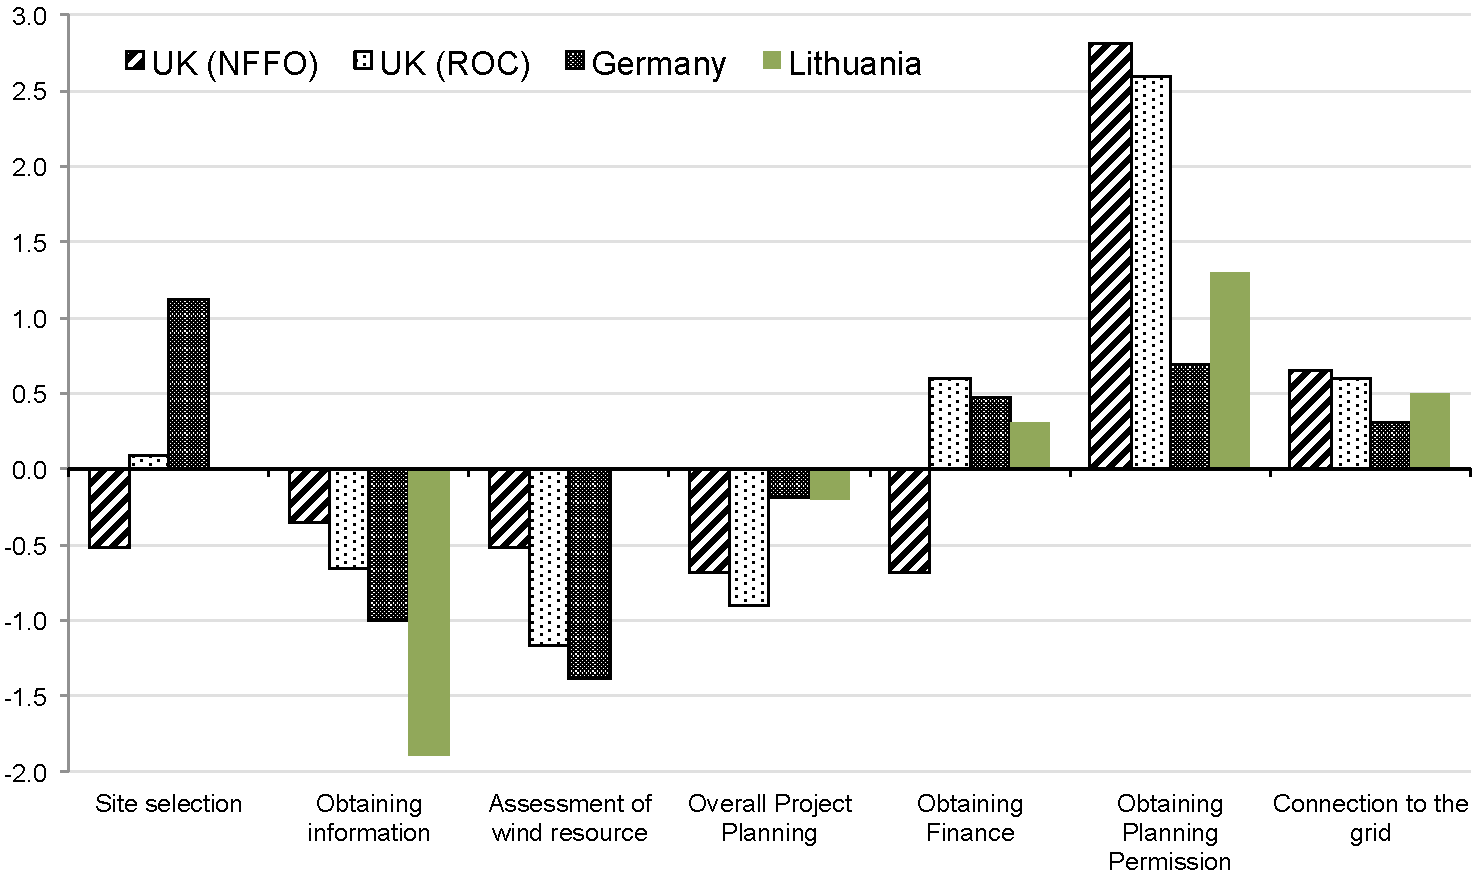
\includegraphics[width=1\textwidth]{fig_survey_barriers}
	\caption{Obstacles to Development: Relative Assessment by Developers}
	\label{fig:fig_survey_barriers}
\end{figure}
% [INSERT FIGURE=... TITLE=Obstacles to Development: Relative Assessment by Developers. SOURCE=Survey, Butler and Neuhoff (2008) NOTE=… ]

Developers reported that they faced no difficulties in finding attractive sites. However they experienced problems when trying to change the land-use category in the municipality district plans, which are updated annually or biannually, but at different dates in different municipalities. This had impact on site selection, and developers favored sites were district plans were soon to be updated. This problem is also mentioned by Marčiukaitis (2011, p. 8 and 12). These slow and complicated bureaucratic procedures will delay the project at least a year. According to Drozdz, Jazepcikas, and Malcolm (2005) there are 9.000 hectare of abandoned land out of 35.000 hectare, showing low demand for it. Compared to Germany, project developers report it easier to find a good site, probably because it is a relatively new industry and specific demand for windy sites is not that high yet.

Respondents did not find any particular difficulties obtaining information. As we see in figure ~\ref{fig:fig_survey_suppliers}, developers report it easier to obtain information in Lithuania, relative to other two countries. This result might also be attributed to the fact that the Butler and Neuhoff survey is from 2004 and developments in information technology has influenced the access and availability of information.

Wind assessment is another problem – our respondents claimed that there are no certified Lithuanian firms that perform wind assessments and that hydrometeorology stations are outdated and cannot be used for wind evaluation. Producers can do valuations themselves, but these are not generally accepted by banks when trying to obtain financial support. Here official or certified reports about wind speeds at specific sites are required (More on wind assessment in the next section).

Obtaining finance under the RO system or in Germany is relatively more difficult than in Lithuania as seen in figure ~\ref{fig:fig_survey_barriers} where we have taken deviation from the average, however the Lithuanian average responses to the difficulties in obtaining finance was 3.7, while only 2.5 and 2.9 respectively under RO and in Germany. Our respondents said that Lithuanian banks and other investors see renewable energy as a risky investment, even under the current feed-in tariff support scheme, where fixed tariff rates are known in advance and guaranteed for 12 years. We believe that Lithuanian banks understand the risks associated with wind power development perfectly well. And that the reasons for difficulty in obtaining finance should instead be attributed to non price related risks: e.g lack of long-term commitments from politicians, risk of time delay when acquiring official documents and certificates, risk of equipment damage (where costly certified repairmen are required to keep warranties intact, and where spare parts will often have to be shipped from non-domestic manufactures), risk of theft, etc. We also believe that banks have had little interest or incentive in providing finance for a new industry, and in Lithuania, unproven technology, and that this will only slowly change as the industry matures and banks become reassured of the repayment. The difference in the length of support between Germany (20 years of support) and Lithuania (12 years) probably also increases costs in Lithuania, as banks will be prone to match loan periods with the official support period. Furthermore only one of our respondents reported that their parent company provided finance, hence it was not a problem for them, while Butler and Neuhoff (2008, p. 1861) report that ``almost half the companies indicated that they had the support of a parent company, making financing easier''. 

The biggest problems developers encountered was obtaining planning permission (average response 4.7) and connecting the plant to the grid (average response 3.8). They describe the problems as time consuming bureaucratic procedures and long lists of required documents that are usually costly to obtain. Some even noted that they didn’t bother to apply for the \emph{40\% discount on connection to grid} available to renewable energy producers, due to cumbersome procedures. In addition they note inconsistencies in long-term policy where laws and requirements change often, leading to additional expenses and delays. In Sawin (2004) long-term policy commitment is mentioned as one of the key factors in policy success, however judging from our survey the Lithuanian government has not yet ensured this.

\subsection{Level of competition}
The second part of the questionnaire helped us to determine the level of competition between developers under the feed-in tariff system, and among those supplying wind project developers. Rating each question on a scale from 0-5; where 0 stands for no competition and 5 for highly competitive market. The average level of competition between project developers and suppliers in Lithuania was 1.9 – that is very close to the Germany (1.96) and UK (1.87) averages. Although the averages are very similar to Germany and the UK, and the variance within each question is small, the variance between the questions is very high in Lithuania, as seen in fig ~\ref{fig:fig_survey_competition} and ~\ref{fig:fig_survey_suppliers}, where Lithuania is located at the extremes of the scale.

\begin{figure}
	\centering
	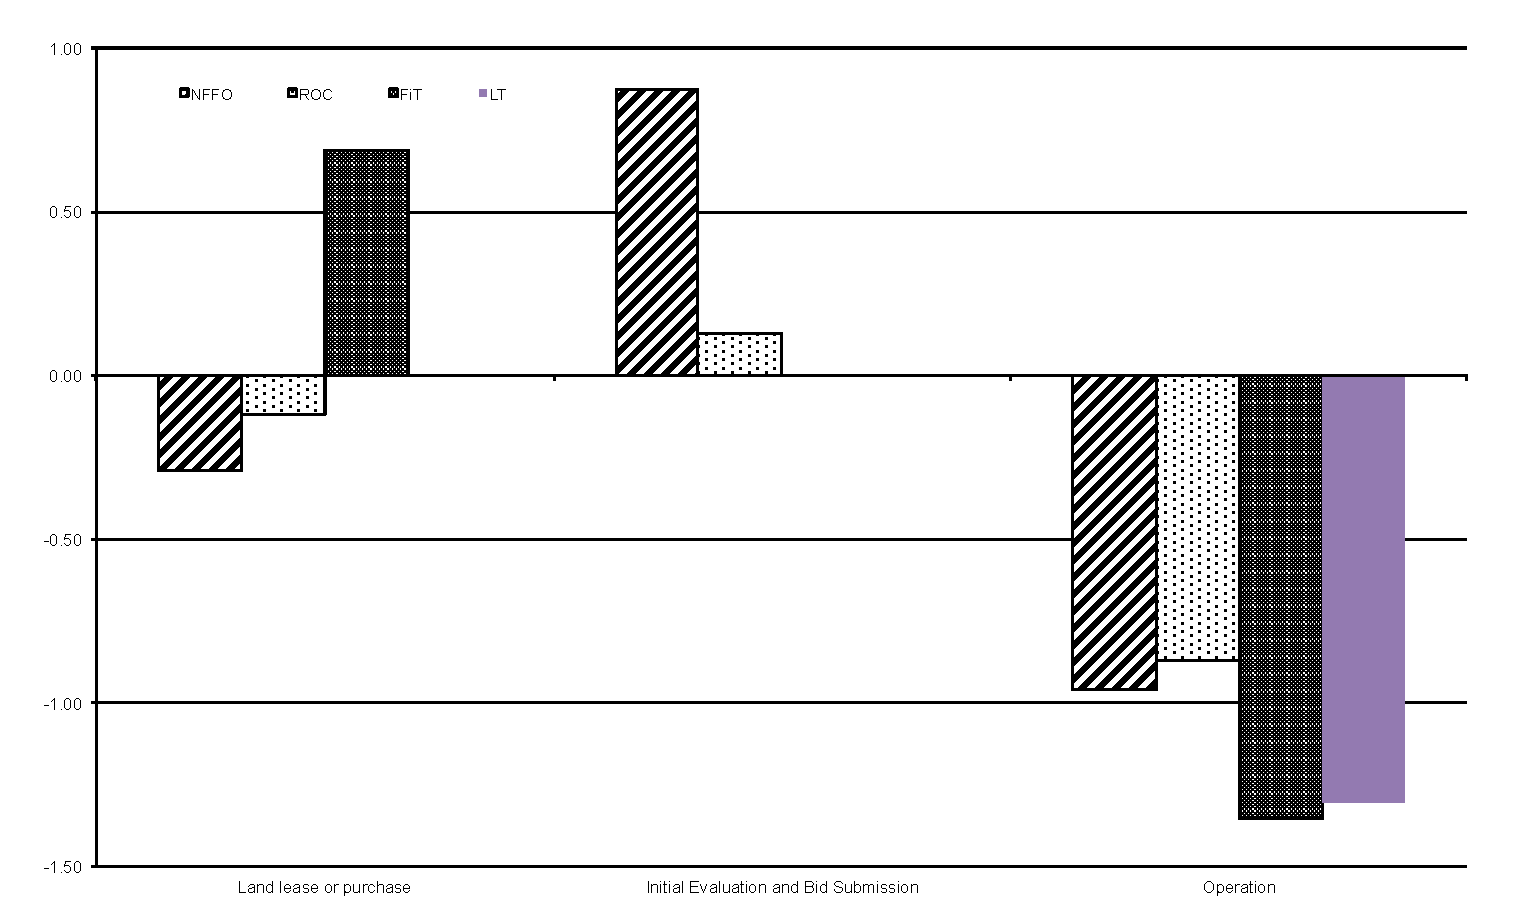
\includegraphics[width=1\textwidth]{fig_survey_competition}
	\caption{Relative Competition Between Developers}
	\label{fig:fig_survey_competition}
\end{figure}
% [INSERT FIGURE=... TITLE=Relative Competition Between Developers SOURCE=Survey, Butler and Neuhoff (2008) NOTE=No Lithuanian data for land lease or purchase and initial evaluation and bid submission]

We chose not to collect the competition scores for land lease or purchase and initial evaluation and bid submission, but instead only a score for operation competition between developers in Lithuania, because of the high availability of land and since Lithuania does not have an auction nor bid system.

Developers report low competition between each other, with an average response of only 0.5, and the Lithuanian and German score is very similar. This can be attributed to the specifics of a feed-in tariff system, where producers do not compete, since they all are guaranteed the fixed price for the duration of the support period. The system fosters cooperation rather than competition. And producers have formed and joined associations of renewable energy producers, that advocate for better conditions and legislations for their businesses. 

\begin{figure}
	\centering
	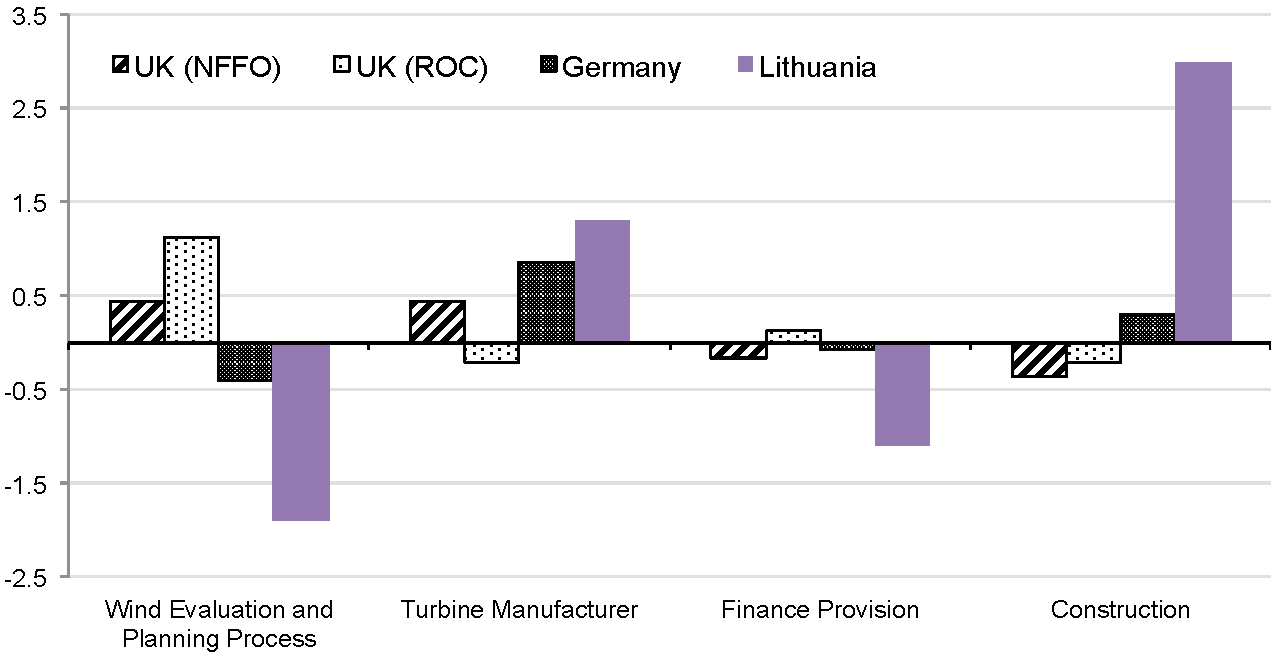
\includegraphics[width=1\textwidth]{fig_survey_suppliers}
	\caption{Relative Competition in Wider Market}
	\label{fig:fig_survey_suppliers}
\end{figure}
% [INSERT FIGURE=... TITLE=Relative Competition in Wider Market SOURCE=Survey, Butler and Neuhoff (2008) NOTE=… ]

We will now evaluate the levels of competition among those supplying wind developers, from the perspective of the project developers. When asking about firms that provide wind evaluation in Lithuania we got an average of zero, since as mentioned earlier there are no firms currently providing this service in Lithuanian. 

Both countries under the feed-in tariff system report lower competition in wind evaluation and planning process than the UK. A possible explanation here might be that under a feed-in tariff system the precise measurement of wind speed is not as important, since network operators are required to accept all of the electricity you generate, this is not the case in the UK. Even with the uncertain initial evaluations you are not exposed to volume risks. This could contributes to the higher prices under the RO system, as developers are forced to do these valuations increasing their initial investment.

The majority of our respondents claimed that the low competition in provision of finance is one of the leading causes of slow renewable energy development. We find that competition on finance provision in Lithuania (average response of 0.8) is much lower than in the two other countries. Part of the explanation here might be that almost all Lithuanian developers had to seek external finance, while about half of the developers in Butler and Neuhoffs survey had support from their parent companies. As we reported earlier few banks proved finance, since they see wind power projects as risky. Swedbank states that they have financed 75\% of all wind farms currently working in Lithuania and this claim just proves low competition in finance provision (Swedbank, 2010). Compare this to the case in Germany where the state bank, Deutsche Ausgleichsbank, provides cheap loans at 0.75\%-2\% below the market price, to renewable energy projects, and reportedly provided finance for 80-90\% of all the wind projects in the 1990s (Butler and Neuhoff 2008, p. 1859 and 1863).

We found very high levels of competition in construction services (average response of 4.8) and high levels of competition in the wind turbine market (average response of 3.2). Developers note that there is no shortage in those two sectors and that new turbine manufactures are still entering the market; which might be a signal that turbine manufacturers see continued potential for wind energy development in Lithuania. 

\subsection{Risks}
We also asked project developers to evaluate the feed-in tariff system and explain the risks they have experienced. The biggest risks, as seen by developers, are risks related to the politics of wind energy and bureaucracy. Project developers see no consistency of long-term policy in Lithuania. And frequently experience regulative changes that are implemented without any lead time with which the industry could adjust to the changes, resulting in high uncertainty. Sawin (2004, p. 26) argues that ``consistency is critical for ensuring continuous growth and stability in the market, enabling the development of a domestic manufacturing industry, reducing the risk of investing in a technology, and making it easier to obtain financing'' and since uncertainty leads to ``cycles of boom and bust in the market. Such cycles lead to suspension of projects, worker lay-offs, and loss of momentum in the industry''.

Another risk noted by project developers is inflation related, as the feed-in tariff rates are currently in nominal values and not automatically adjusted for inflation. In 2009 and 2012 the feed-in tariff rates for new builds were adjusted for inflation, by parliament, who changed the Renewable Energy Law. However these changes are discrete and no official commitment has been made ensuring its continuity. This could potentially also be a problem in Germany were the rates are also in nominal values, however the german central bank’s track record of keeping the inflation rate just below 2\% is much better than that of the Lithuanian Central bank. As seen from 2005 to 2011 where the Lithuanian harmonised index of consumer prices increased from 100 to 133.9 leading to huge decrease in real wind energy price, since the 12-year guaranteed tariffs are non inflation adjusted (EUROSTAT prc\_hicp\_aind). As Bauknecht, Connor and Mitchell (2006, p. 301) note on price risks, developers can use hedging, pay a premium, and convert price fluctuation into a certain price band or fixed amount, this will reduce the price risk but also represents an additional cost, but ``as many renewable generators are small generators, they tend to be relatively risk averse due to a less diverse fuel portfolio and a limited ability to finance projects through the balance sheet. They are therefore likely to be disadvantaged by high-risk markets ... They are therefore likely to pay relatively high hedging fees for reducing their risk to a minimum''. Hence the case could be made for inflation-index feed-in tariffs in Lithuania, as a way to further reduce risks, and thereby lower costs. This \emph{risk} may however be more of a theoretical possibility than an actual problem. Weitzel (2012, p. 486) in his comment on the differences between the feed-in system of Germany and that of Ontario, where feed-in tariff rates are actually inflation-linked, conclude that ``the NPV an investor requires in Ontario should ceteris paribus be lower than in Germany, as the investment would be -less risky in terms of inflation risk. This is however not observed in the data''. The data shows that the remuneration levels are higher in Ontario than they are in Germany.

\section{Perspectives on the future}
Before concluding on the findings of our paper we will shortly discuss the latest developments and future perspectives in Lithuania.

After the closure of Ignalina nuclear power plant Lithuania decided to start the planning of a new nuclear power plant in Visaginas (Ministry of Energy 2012. National Energy Independence Strategy 2012). The new power plant is supposed to solve the energy deficit created in the Baltic region after closing the Ignalina nuclear power plant. However simultaneously with the parliamentary election held on 14. October 2012, there has been a referendum on the new nuclear power plant. The results of the referendum was 65\% voting against (35\% voting in favor) of the creation of a new nuclear power plant (CEC 2012). This result creates a huge discrepancy between the public opinion and the long-term national strategies pursued. And cast further uncertainty over the creation of the Visaginas nuclear power plant. Moreover the National Energy Independence Strategy (2012) and supporting legislation has been based on a new nuclear power plant planned to open 2020. This new development will therefore most likely impact renewable energy policy too.

The feed-in tariff system will be heavily adjusted. The planning is well under way, but yet without a planned amendment date. The current feed-in tariff system will be combined with an auction mechanism, where the maximum auction price accepted will be calculated similarly to how the feed-in tariff rate is currently calculated. The new system will divide Lithuania into six regions and specify capacity limits (MW) for each region. An auction takes place for each region, and producers compete in providing the lowest price, which if they win will then be used as feed-in tariff rate in that region. Only projects that have been built or are in the process of being build can participate in the auction (NCC 2011, section IV, clause 28.3). And after the auction all participants have opportunity to accept the winning auction rate for 12 years. The auctions are held every quarter or half-year until the capacity limit of that region has been reached. Essentially the new system will offer the same rate as currently, unless producers through the auction indicate that they are able to develop at a lower cost. The overall aim is to ensure that development happens at the lowest possible cost.

The new system will solve two problems: 1) It will introduce price differentiation based on different wind speeds, by splitting rates up by region (as mentioned earlier there are large differences on wind speeds in the coastal region and the eastern and southeastern part of Lithuanian). 2) It should solve the technical wind energy capacity problems, discussed in Katinas (2007). As mentioned earlier there is capacity limit of 500 MW for wind power in Lithuania, this barrier is however unevenly distributed across the country, with different regions having different capacity limits due to the capacity of their transmission stations, the new system will account for those differences.

The new system might also cause some new, and unintended problems. The final tariff rates will be less predictable, most likely leading to increases in the risk of investment. Making it harder and/or more costly to obtain finance. And note here that we have already shown with our survey that current opportunities to obtain finance is perceived as a major obstacle by project developers.

Moreover price competition can lead to an inflow of cheap and low-quality wind turbines that are noisier. This can have a negative impact on neighbouring communities and also on the overall acceptance of wind energy, and complicate future development. Marčiukaitis (2011, p.10) report that Lithuanians currently have positive attitudes towards wind energy, so long as they are not constructed in their neighborhood. 

Project developers will naturally perceive the new system as an deterioration, since they face lower prices compared to the current system. And this is also mainly the reponds we got in our survey, however project developers also claimed that new system will have a negative impact due to increase in price associated risks, as discussed above. 

The lessons learned in the UK might indicate other likely problems with the new system. Dow and Wood (2011, p. 2229) explains why the NFFO system (and also to some extent the RO system) has not worked as intended. They list the failures as; ``finite and limited duration of subsidies due to limited mechanism lifespan, excessive focus on competition and low costs, mechanism uncertainty, unresolved planning and electricity grid network issues and policy uncertainty/excessive change''. Here we will only shortly discuss the first, as some of others have already been discussed, and some do not apply to the new Lithuanian system. 

If we take a longer view beyond the current capacity limits in Lithuania, then limited mechanism lifespan is likely to arise. Once the initial capacity limits has been reached, currently estimated at 2017 (National Energy Independence Strategy 2012), and once extending this limit becomes a possibility (for whatever technical reason), wind development will enter go and bust-cycles, characterised by uncertainty of when new bidding rounds will occur and irregular intervals between regional capacity limits being extended - similar to those experienced under the NFFO auction system, and also in the US when the ``U.S. Production Tax Credit for wind energy has been allowed to expire several times, only to be extended months later'' (Sawin 2004, p. 26). 

We do not believe the new system in Lithuania will suffer from an excessive focus on competition and low costs although it remains a possibility. But splitting the country up into regions and only accepting auction offers from ready-built, and unconnected projects or projects under construction, could end in very low auction participation rates. As we mentioned earlier only 41 projects have been built since 2002. The new system proposes to restrict developers to installing a maximum of 40\% of the regions capacity limit (NCC 2011, section VII, clause 72), which might inhabit economies of scale and the efficiency gains that follow from it.

\section{Conclusion}
Our paper investigates the current renewable policy in Lithuania with comparison to Germany and the United Kingdom. We found that Lithuania managed to achieve low costs, similar to Germany and lower than the UK through their feed-in tariff system, contrary to economic theory where you would expect lower prices when producers are exposed to price competition. But since a feed-in tariff system is exempted from price-, volume- and balancing-risks it manages to achieve higher efficiency and lower price. Lithuania experienced relatively fast development of wind energy and quickly caught up to level of development in the UK. However Lithuanian has not yet reached the level of development in Germany. We argue that is attributed as follows: 1) to differences within the feed-in tariff system, such as tariffs differentiated for wind speeds, and differences in support period. 2) and to country specific problems; obtaining finance, lack of long term policy commitments, high inflation, and lack of wind evaluation providers. In closing we can say that Lithuania has had a good and well thought financial support mechanism that reduced costs, but the surrounding ecosystem and external factors have restricted development from reaching even greater levels. We see room for improvement in current legislation and planning procedures, that could lead to higher deployment levels of wind power, and that the new feed-in tariff system will solve some of the current problems, but also increase uncertainty and risks which might lead to higher costs down the road.

\section{References}
...

\section{Appendix A}
% [INSERT PAGE=Feed-in-tariffs-rates.pdf TITLE=The onshore wind power feed-in tariff rates in Germany (1991-2030) SOURCE=BMU (EEG 2000, section 7. EEG 2004, article 10. EEG 2009, section 20, 29 and 30. EEG 2012, section 20, 29 and 30). Lauber and Mez (2004). NOTES=* StrEG: 90\% of sales price. ** EEG 2000: Operation time of prior installation is halved (min. 4 years). After that follow same reduction of rate rules as new installations. *** EEG 2000: Degression from 2002. **** EEG 2012: Small-scale (≤50KW) will recieve initial fee for 20 years.]

\section{Appendix B. Questionnaire}
Complete survey questionnaire.

\section{Appendix C. Policy timeline}
The policy timeline.





% Which P did and Which did jonas do.





\end{document}